\documentclass{article}
\usepackage[english]{babel}
\usepackage[utf8]{inputenc}
\usepackage[parfill]{parskip}
\usepackage{amsmath,amssymb,amsthm}
\usepackage{a4wide}
\usepackage{color}
\usepackage{graphicx}

\newcommand{\eps}{\varepsilon}
\newcommand{\bigo}[1]{\mathcal{O}\left(#1\right)}
\newcommand{\note}[1]{\emph{\color{blue}#1}}
\renewcommand{\L}{\mathcal{ L}}
\newcommand{\R}{\mathbb{ R}}
\newcommand{\N}{\mathbb{ N}}
\newtheorem{defin}{Definition}
\newtheorem{prop}{Property}

\renewcommand{\H}{\mathcal{ H}}
\newcommand{\B}{\mathcal{ B}}
\newcommand{\dealii}{deal.ii{}}
\renewcommand{\P}{\mathbb{ P}}
\newcommand{\K}{\mathcal{ K}}
\newcommand{\V}{\mathcal{ V}}
\title{Activity report for Omar\textsuperscript{2} collaboration in Sussex}
\author{Omar Richardson}

\begin{document}
\maketitle

\section{Introduction}
This report contains a summary on the activities during a four-week research visit to the MPS in the University of Sussex, where Omar Richardson collaborated with Omar Lakkis and Chandrasekhar Venkataraman.

This report is structured as follows. Section~\ref{sec:problem} describes the problem under consideration. Section~\ref{sec:space} proposes a space discretization for the aforementioned problem, while Section~\ref{sec:time} suggests a time discretization. Section~\ref{sec:dealii} provides some detail on the finite element library deal.ii and describes what should be considered while implementing a multiscale finite element problem. In Section~\ref{sec:manufactured}, we present a manufactured problem of which we know a priori know the exact solution.
Finally, Section~\ref{sec:adaptivity} describes some possible routes forward regarding adaptivity.

\section{Problem description}
\label{sec:problem}

We consider the following problem, posed on two spatial scales $\Omega\subset \R^{d_1}$ and $Y \subset \R^{d_2}$ with $d_1,d_2 \in \{1,2,3\}$ in time interval $t\in S := (0,T)$ for some $T>0$. Find the two \emph{pressures} $\pi: S\times\Omega \to \R $ and $\rho: S\times\Omega\times Y\to \R$ that satisfy:

\begin{align}
    \label{eq:main_ellip}&-A\Delta_x\pi=f(\pi,\rho)  &\mbox{ in }S\times\Omega,\\
    \label{eq:main_para}&\partial_t\rho-D\Delta_y\rho = 0  &\mbox{ in }S\times\Omega\times Y,\\
    \label{eq:main_robin}&D\nabla_y\rho\cdot n_y= k(\pi+p_F-R\rho)&\mbox{ in } S\times\Omega\times\Gamma_R,\\
    \label{eq:main_neumann}&D\nabla_y\rho\cdot n_y=0&\mbox{ in }S\times\Omega\times\Gamma_N,\\
    \label{eq:main_dirichlet}&\pi=0 &\mbox{ in }S\times\partial\Omega,\\
    \label{eq:main_initial}&\rho(0,x,y)=\rho_I(x,y)&\mbox{ in } \overline{\Omega\times Y},
\end{align}
where $\Gamma_R \cup \Gamma_N = \partial Y$, $\Gamma_R \cap \Gamma_N = \emptyset$ and $f:S\times\Omega\times Y \to \R$ is a function. We refer to \eqref{eq:main_ellip}-\eqref{eq:main_initial} as ($P_1$).


\subsection{Weak solutions}

We are interested in solutions to ($P_1$) in the weak sense. This is motivated by the fact that the underlying structured media can be of composite type, allowing for discontinuities in the model parameters.

\begin{defin}[Weak solution]
    A weak solution of ($P_1$) is a pair
    \begin{equation*}
        (\pi,\rho)\in\L^2(S;\H_0^1(\Omega))\times \L^2(S;\L^2(\Omega;\H^1(Y)))\cap \H^1(S;\L^2(\Omega;\L^2(Y)))
    \end{equation*}
    that satisfies for all test functions $(\varphi,\psi) \in \H^1_0(\Omega)\times \L^2(\Omega;\H^1(Y))$ the identities

\begin{equation}
    \label{eq:weak_pi_cont}
    A\int_\Omega\nabla_x\pi\cdot\nabla_x\varphi dx=\int_\Omega f(\pi,\rho)\varphi dx,
\end{equation}
and
\begin{equation}
    \label{eq:weak_rho_cont}
    \int_\Omega\int_Y\partial_t\rho\psi dydx+D\int_\Omega \int_Y\nabla_y \rho\cdot\nabla_y\psi dydx= \kappa\int_\Omega\int_{\Gamma_R}(\pi+p_F-R\rho)\psi d\sigma_ydx,
\end{equation}
for almost every $t \in S$ .
\end{defin}

\section{Space discretization}
\label{sec:space}
In this section we prove that ($P_1$) has a weak solution by approximating it with a Galerkin projection.
We show the projection exists and is unique, and proceed by proving it converges to the weak solution of ($P_1$).
First, we introduce the necessary tools for defining the Galerkin approximation.

We use one mesh partition for each of the two spatial scales.
Let $\B_H$ be a mesh partition for $\Omega$ consisting of simplices. We denote the diameter of an element $B \in \B_H$ with $H_B$, and the global mesh size with $H:= \max_{B \in \B_H} H_B$.
We introduce a similar mesh partition $\K_h$ for $Y$ with global mesh size $h:= \max_{K \in \K_h} h_K$.

Let $l\in \N$ be the order of the finite element spaces.
Our macroscopic and microscopic finite element spaces $V_H$ and $W_h$ are defined as, respectively:
\begin{align*}
    V_H &:= \left\{ \left. v \in C^0(\Omega)\right|\,v|_B \in \P^l(B) \mbox{ for all } B \in \B_H  \right\},\\
        W_h &:= \left\{ \left. w \in C^0(Y)\right|\,w|_K \in \P^l(K) \mbox{ for all } K \in \K_h  \right\}.
\end{align*}
where $\P^k(W)$ denotes the function space of polynomials of degree $k$ on set $W$.

Let $\langle \xi_B \rangle_{\B_H}:= \operatorname{span}(V_H)$ and $ \langle \eta_K \rangle_{\K_h}:= \operatorname{span}(W_h)$ defined such that
\begin{equation}
    \xi_j(x_i) = \eta_j(y_i) = \delta_{ij},
\end{equation}

and let $\alpha_B,\beta_{BK} : S \to \R$ denote the Galerkin projection coefficient for a patch $B$ and $B\times K$, respectively. We introduce the following Galerkin approximations of the functions $\pi$ and $\rho$:
\begin{equation}
    \begin{split}
        \pi^H(t,x) &:= \sum_{B \in \B_H} \alpha_B(t) \xi_B(x),\\
        \rho^{H,h}(t,x,y) &:= \sum_{B \in \B_H, K \in \K_h} \beta_{BK}(t) \xi_B(x) \eta_K(y),
    \end{split}
    \label{eq:trunc}
\end{equation}
where we clamp $\alpha_B(t)=0$ for all $B\in \B_H$ with $\partial B \cap \partial \Omega\neq \emptyset $ to represent the macroscopic Dirichlet boundary condition.

Reducing the space of test functions to $V^H$ and $W^h$, we obtain the following discrete weak formulation: find a solution pair
\[(\pi^H(t,x),\rho^{H,h}(t,x,y)) \in \L^2(S;V^H)\times \L^2(S;V^H\times W^h)\] that are solutions to
\begin{equation}
    \label{eq:weak_pi}
    A\int_\Omega\nabla_x\pi^H\cdot\nabla_x\varphi dx=\int_\Omega f(\pi^H,\rho^{H,h})\varphi dx,
\end{equation}
and
\begin{equation}
    \label{eq:weak_rho}
    \begin{split}
    &\int_\Omega\int_Y\partial_t\rho^{H,h}\psi dydx+D\int_\Omega \int_Y\nabla_y \rho^{H,h}\cdot\nabla_y\psi dydx\\
    &\quad= \kappa\int_\Omega\int_{\Gamma_R}(\pi^H+p_F-R\rho^{H,h})\psi d\sigma_ydx,
    \end{split}
\end{equation}
for any $\varphi \in V_H$ and $\psi \in V_H \times W_h$ and almost every $t \in S$.

These concepts lead us to the first proposition.
\ \\
\begin{prop}[Existence and uniqueness of the Galerkin approximation]
    \label{prop:ex_un}
    There exists a unique solution $(\pi^H,\rho^{H,h})$ to the system in \eqref{eq:weak_pi}-\eqref{eq:weak_rho}.
\end{prop}
\begin{proof}
    The proof is divided in three steps.  In step 1, the local existence in time is proven. In step 2, global existence in time is proven. Step 3 is concerned with proving the uniqueness of the system.

    We introduce an integer index for $\alpha_B(t)$ and $\beta_{BK}(t)$ to increase the legibility of arguments in this proof.
    Let $N_1 := \{1,\dots, |\B_H|\}$ and $N_2 := \{1,\dots, |\K_h|\}$. We introduce bijective mappings $n_1:N_1\to \B_H$ and $n_2: N_2 \to \K_h$, so that each index $j\in N_1$ corresponds to an element $B \in \B_H$ and each index $k\in N_2$ corresponds to a $K \in \K_h$.

    \textit{Step 1: local existence of solutions to \eqref{eq:weak_pi} - \eqref{eq:weak_rho}}:
    By substituting $\varphi = \xi_i$ and $\psi = \xi_i\eta_k$ for $i\in N_1$ and $k\in N_2$ in \eqref{eq:weak_pi}-\eqref{eq:weak_rho} we obtain the following system of ordinary differential equations coupled with algebraic equations.

    \begin{align}
        \sum_{j\in N_1} P_{ij} \alpha_j(t) &= F_i(\alpha,\beta)\label{eq:ode_alpha} \mbox{ for }i\in N_1,\\
        \beta^\prime_{ik}(t) + \sum_{j\in N_1,l\in N_2} Q_{ijkl} \beta_{jl}(t) &= c_{ik} + \sum_{j\in N_1} E_{ijk}\alpha_j\label{eq:ode_beta}\mbox{ for }i\in N_1\mbox{ and }k \in N_2,
    \end{align}
    with
    \begin{equation}
        \begin{split}
            P_{ij} &:= A \int_\Omega \nabla_x \xi_i \cdot \nabla_x \xi_j\,dx,\\
            F_i &:= \int_\Omega f \left( \sum_{j\in N_1}\alpha_j(t) \xi_j,\sum_{j\in N_1,l\in N_2}\beta_{jl}(t)\xi_j\eta_l \right)\xi_i\,dx,\\
            Q_{ijkl} &:= D \int_\Omega \xi_i\xi_jdx\int_{Y} \nabla_y \eta_k\cdot \nabla_y \eta_ldy + \kappa R\int_\Omega \xi_i\xi_j dx\int_{\Gamma_R}\eta_k \eta_ld\sigma_y,\\
            E_{ijk} &:= \kappa\int_\Omega\xi_i\xi_j dx\int_{\Gamma_R} \eta_kd\sigma_y,\\
            c_{ik}&:= \kappa p_F\int_\Omega \xi_i dx\int_{\Gamma_R} \eta_k d\sigma_y\,
        \end{split}
        \label{eq:matrices}
    \end{equation}
    Applying \eqref{eq:main_initial} to \eqref{eq:weak_pi} and \eqref{eq:weak_rho} yields:
    \begin{equation}
        \begin{split}
            \alpha_i(0) &= \int_\Omega \xi_i\pi_I\,dx,\\
            \beta_{ik}(0) &= \int_\Omega\int_Y\xi_i\eta_k\rho_Idydx.
        \end{split}
        \label{eq:fem_init}
    \end{equation}

    For all $t \in S$, the coefficients $\alpha_i(t), \beta_{ik}(t)$ of \eqref{eq:trunc} are determined by \eqref{eq:ode_alpha}, \eqref{eq:ode_beta} and \eqref{eq:fem_init}.
\end{proof}

\section{Time discretization}
\label{sec:time}
Implementation of this scheme requires a discretization of $\alpha_i(t)$ and $\beta_{ik}(t)$ in \eqref{eq:ode_alpha}-\eqref{eq:ode_beta}.

In this section, we propose a mix of explicit and implicit first order time integration. Assuming the notation and variables from the previous section, we propose the following scheme:

Let $\Delta t>0$ be fixed, and let $\alpha_i^n := \alpha_i(n\Delta t)$ and $\beta_{ij}^n := \beta_{ik}(n\Delta t)$ for any $i\in N_1$, $j \in N_2$ and $n\geq0$. Then, given some $\alpha_i^0$ and $\beta_{ik}^0$ we obtain the following scheme:
\begin{align}
    \sum_{j\in N_1} P_{ij} \alpha_j^n &= F_i(\alpha^{n-1},\beta^{n-1})\label{eq:discr_alpha} \mbox{ for }i\in N_1,\\
    \beta_{ik}^{n} + \Delta t\sum_{j\in N_1,l\in N_2} Q_{ijkl} \beta_{jl}^{n} &= \beta_{ik}^{n-1} + \Delta tc_{ik} + \Delta t\sum_{j\in N_1} E_{ijk}\alpha_j^{n-1}\label{eq:discr_beta}\mbox{ for }i\in N_1\mbox{ and }k \in N_2,
\end{align}

This time discretization is explicit in the macroscopic equation and implicit in the microscopic equation. This avoids approximating the nonlinear term $f$, and ensures (hopefully) more stability in the microscopic equation without much of a cost, since this equation is linear.

Convergence of this scheme is as of now still an open problem.

\section{deal.II}
\label{sec:dealii}

Finite element library deal.ii is a C++ library that is able to solve finite element problems. It is an open source library that is under active development. Selling points are its dimension independent implementation formulation, its support for many different kinds of finite elements and the possibility for grid refinement. Possible issues are its restriction to quadrilaterals and the fact that some routines are implemented in a black-box-like manner.

\subsection{Implementation structure}
Implementations in deal.II follow the object-oriented paradigm. This means that mathematical concepts like functions, solution approximations, boundary conditions, matrices, grids and triangulations are represented with instances of deal.II objects.

Most finite element codes in deal.II is roughly structured in the same way:

\begin{enumerate}
    \item Create a domain and a ``triangulation'' of that domain.
    \item Distribute the degrees of freedom based on the triangulation and the degree of finite elements.
    \item Initialize the system matrix and the right hand side and solution vector.
    \item Assemble the system by looping over cells and integrate the discrete weak form per cell.
    \item Interpolate and apply the boundary conditions.
    \item Solve the system, either directly or iteratively.
    \item Post-process and output the solution.
\end{enumerate}



\subsection{Multiscale implementations}
When one tries to solve a multiscale finite element problem numerically, it is important to consider how the implementation will be structured.
Doing it naively can lead to a computational effort which would exceed the single scale problem, i.e. creating a micro-problem for each degree of freedom on the macroscopic grid.
Luckily, most problems allow for a reuse of objects and structures, saving both memory and computational effort.

For our multiscale problem, we suggest the following improvements over said naive implementation. Some of these improvements rely on assumptions which will no longer hold in more general or more complicated cases. In that case, they will be revised when necessary.
\begin{itemize}
    \item Share among all microscopic instances: the microscopic grid, triangulation, degree of freedoms and the sparsity pattern of the system matrix.
    \item Create one microscopic system for each macroscopic cell, where we can easily interpolate the required value of $\pi$.
\end{itemize}

In order to create a two-way information exchange between the microscopic and macroscopic grid, we require some technicalities in our implementation.

Because each microscopic system is defined for a macroscopic cell, we associate a specific local value of $\pi$ with each system: the finite element function value for the mid-point of the cell.
By using mid-point quadrature integration techniques, we are able to derive this value from the finite element solution of $\pi$.

The right hand side of the macroscopic system requires the integral of $\rho$ over $Y$. Using a second-order gaussian integration technique we obtain a value of this right hand side for each cell center.
An improvement would be to interpolate these central cell values to all quadrature points.
This could be done by either (1) creating a microscopic grid for each quadrature point, although that has the drawback that the order of integration heavily impacts the computational load, or (2) using a linear interpolation technique to obtain a better approximation of the right hand side in the quadrature points, although that cannot (reliable) be extended to higher order interpolation.

In the present implementation, however, we find solace in the fact that this piecewise constant approximation of the right hand side function is still a consistent one.
\section{Manufactured problem with solutions}

\subsection{Problem description}
\label{sub:problem_description}

\label{sec:manufactured}
In this section we propose a multiscale PDE with two-way coupling of which we know the exact solution. We use this system to test our implementation and see if the scheme we use converges with the desired order.

Let us assume the same notation as in Section~\ref{sec:problem}.
Now, we are looking for a pair of solutions $(\pi(x),\rho(x,y))$ that solve the following system:
\begin{align}
    \label{eq:man_ellip}&-\Delta_x \pi(x) = \int_Y \rho(x,y) dy &\mbox{ in } \Omega\\
    \label{eq:man_para}&- \Delta_y \rho(x,y) = -p(x)\Delta_y r(y) &\mbox{ in }  \Omega\times Y \\
    \label{eq:man_ell_bc}&\pi(x) = p(x)  &\mbox{ on } \partial \Omega \\
    \label{eq:man_para_bc}&\rho(x,y) = p(x)r(y) &\mbox{ on } \Omega \times \partial Y
\end{align}
for some $p(x)$ and $r(y)$.
For the rest of this discussion, we fix $\Omega = [0,1]^2$, $Y = [0,1]^2$, $p(x) = \cos(x_1) + \sin(x_2)$ and $r(y) = y_1^2 + y_2^2$.
This results in the solution pair:
\begin{equation}
    \pi(x) =  \cos(x_1) + \sin(x_2),\quad \rho(x,y) = \left( \cos(x_1) + \sin(x_2) \right) \left(  y_1^2 + y_2^2 \right)
\end{equation}

We use deal.II to solve the provided system. We do so by an iterative scheme; take an initial guess for the macroscopic solution (for instance, $\pi=1$), and using this as data to solve the microscopic systems.
Then, take the solutions of the microscopic systems as data and solve the macroscopic system.
Repeat this process until the difference in subsequent solution approximations no longer exceeds a specified tolerance.

\subsection{Convergence}
To assess the quality of this implementation, we use the following three tests:
\begin{enumerate}
    \item Test the convergence of the microscopic scheme, given the correct macroscopic solution
    \item Test the convergence of the macroscopic scheme, given the correct microscopic solution
    \item Test the convergence of the full multiscale system, both in number of iterations as in the grid points.
\end{enumerate}

In Figure~\ref{fig:micro_convergence}, we see a standard quadratic convergence for the $\L^2$ error and linear convergence for the $\H^1$ error, in line with the standard finite element error estimates.

\begin{figure}[ht]
    \centering
    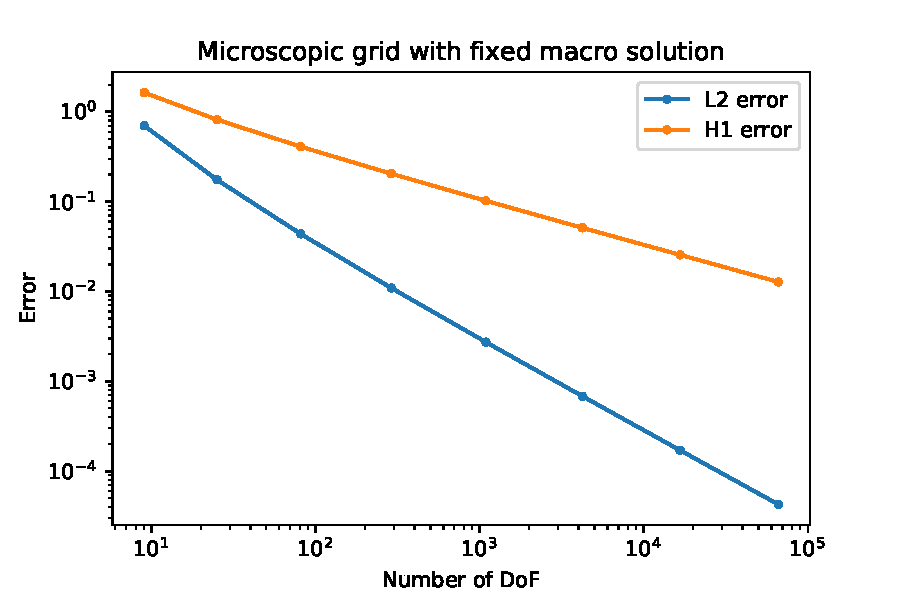
\includegraphics[width=0.8\textwidth]{micro_convergence.pdf}
    \caption{$\L^2$ and $\H^1$ errors of the microscopic scheme as a function of the number of degrees of freedom in a log-log plot.}
    \label{fig:micro_convergence}
\end{figure}

This same behaviour is illustrated in Figure~\ref{fig:macro_convergence}.

\begin{figure}[ht]
    \centering
    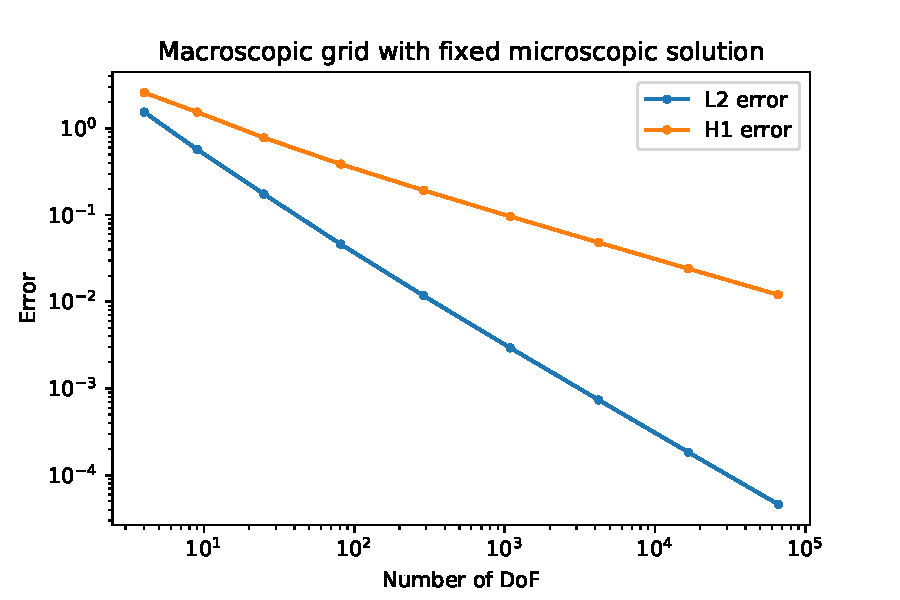
\includegraphics[width=0.8\textwidth]{macro_convergence.pdf}
    \caption{$\L^2$ and $\H^1$ errors of the macroscopic scheme as a function of the number of degrees of freedom in a log-log plot.}
    \label{fig:macro_convergence}
\end{figure}

Subsequently, in Figure~\ref{fig:multiscale_macro} and Figure~\ref{fig:multiscale_micro}, we observe convergence of the full multiscale system.
Notice how in the macroscopic equation, each subsequent iteration decreases the error by a seemingly fixed amount, while in the microscopic equation, convergence does not always occur monotonously.

Also notice how the rate of convergence in the $\L^2$ norm is not maintained in the largest grid, due to what seems a lack of iterations.
A third interesting observation is the seemingly quadratic convergence of the $\H^1$ error in the microscopic system. The reason for this is still to be analysed.

Finally, observe how in the microscopic system, the error of the first iteration reduces as the number of degrees of freedom increases. This occurs because we solve the macroscopic equation before we solve the microscopic one, therefore having better initial data as the macroscopic equation does.
For higher grid resolution, an increasing minimum number of iterations is necessary to obtain the the highest accuracy. Regardless, convergence is largely as expected.

\begin{figure}[ht]
    \centering
    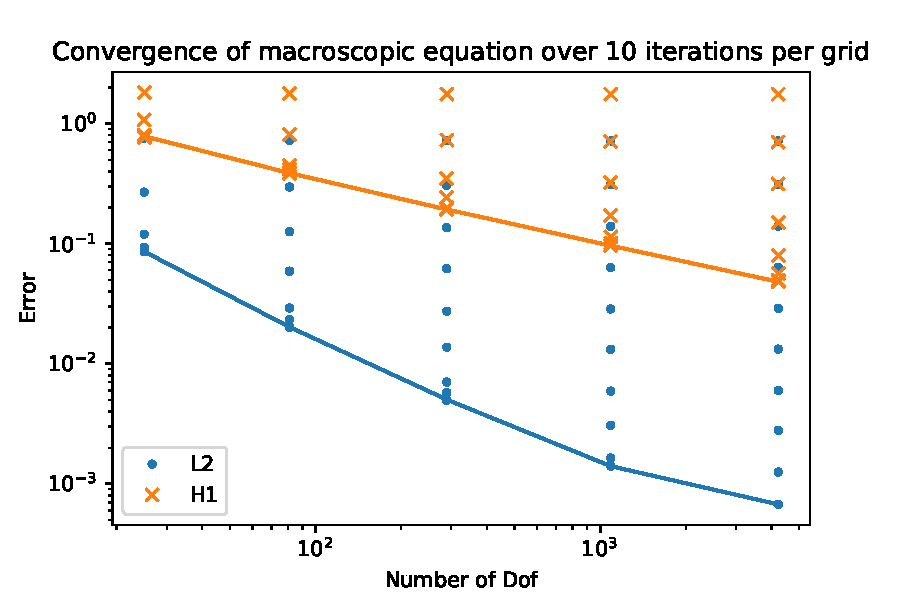
\includegraphics[width=0.8\textwidth]{multiscale_macro.pdf}
    \caption{$\L^2$ and $\H^1$ errors of the macroscopic part of the multiscale equation as a function of the number of degrees of freedom, log-log plot. Each point corresponds to an iteration, the line corresponds to the final iteration.}
    \label{fig:multiscale_macro}
\end{figure}

\begin{figure}[ht]
    \centering
    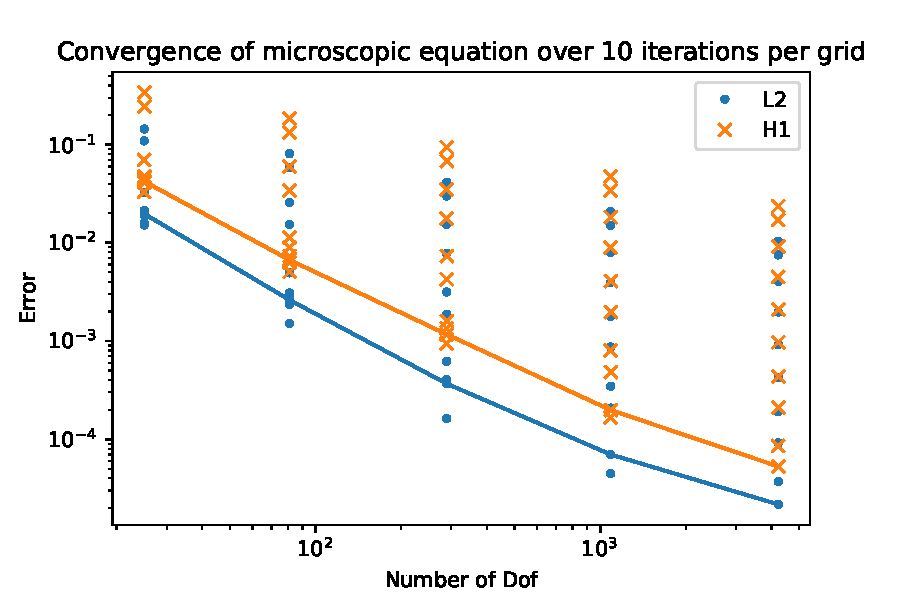
\includegraphics[width=0.8\textwidth]{multiscale_micro.pdf}
    \caption{$\L^2$ and $\H^1$ errors of the macroscopic part of the multiscale equation as a function of the number of degrees of freedom, log-log plot. Each point corresponds to an iteration, the line corresponds to the final iteration.}
    \label{fig:multiscale_micro}
\end{figure}

\section{Future work: Concepts for adaptivity}
\label{sec:adaptivity}

In this section, we shortly describe three possible strategies that can increase the accuracy of this finite element scheme, based on a posteriori error indicators.
One of the goals is to find out which of these strategies produces the highest accuracy, given the same amount of computational power.
Each of these strategies is based on microscopic refinement; the macroscopic mesh is left as is.
As a microscopic error indicator, we use $\eta(x,y)$, defined only for $x \in \Omega$ which correspond to vertices on the discretization of $\Omega$ and $y \in Y$ which correspond to elements on the discretization of $Y$.
As a macroscopic error indicator, we use $\xi(x)$, similarly defined.

\subsection{Maximum error minimization}
\label{sec:max_min}
This strategy is based on the desire to use one microscopic grid for all microscopic systems.
We compute the microscopic error indicator for each microscopic element, but collapse them to fit on a single microscopic grid by maximizing over all macroscopic vertices, i.e., we define a single error indicator $\tilde{\eta}:Y \to \R$ as:
\begin{equation}
    \tilde{\eta}(y) := \max_{x\in \Omega} \eta(x,y),
\end{equation}
and we use this error indicator to decide on refinement for all microscopic grids.
This way, we are able to reuse the same microscopic grid for all microscopic systems, all the while still being able to make guarantees on the upper bound of the error.
\subsection{Error grouping}
\label{sec:error_grouping}
The first approach is memory-efficient, but might refine microscopic systems in locations where it is not necessary and for that reason become computationally inefficient.
For this reason, we propose a generalization that can compromise between memory usage and CPU usage.
We drop the requirement that all microscopic systems have the same microscopic grid and instead introduce $n$ possibly different grids.
After the first iteration, we group the microscopic error indicators on similarity into $n$ different groups (how to do this is not trivial), and for each group, create a new grid (and corresponding data structures).
This grid will be a refinement of the previous grid based on the collapsed error indicator of its group.

Things to keep in mind when grouping error indicators is not only error magnitude, but also error localisation.

\subsection{Macro-based micro error indicators}
As a last option, we drop any restrictions on microscopic grid similarity and instead try to not only minimize microscopic errors but also macroscopic ones, by refining the microscopic grid in locations where it contributes to a larger macroscopic error, giving rise to the following refinement strategy: Given a threshold $\bar{\eta}= \bar{\eta}(\xi(x))$, refine the microscopic grid when
\begin{equation}
    \eta(x,y) > \bar{\eta}(\xi(x))
\end{equation}
where the relation between $\bar{\eta}$ on $\xi$ has to be explored.
\bibliography{literature}
\bibliographystyle{ieeetr}
\end{document}
